\documentclass[12pt]{article}
\usepackage{graphicx}
\usepackage{subcaption}
\usepackage{mwe}
\usepackage[]{mcode}
%\usepackage{lingmacros}
%\usepackage{tree-dvips}
%\usepackage{blindtext}
%\usepackage[utf8]{inputenc}
\begin{document}

\title{ENPM673 - P2}
\author{Gudjon Einar Magnusson}

\maketitle

\section{Lane Detection}

For lane detection I used inverse perspective mapping (IPM) to rectify the road ahead and get what looks like a top down view of the road. For simplification I assumed a fixed view forming a trapezoid from the bottom corners towards the center of the frame. I hard coded the horizon to be a few pixels below the center of the frame. These hard assumptions made it easy to implement but unfortunately it is not very robust against changes in landscape. Ideally I would like to detect the vanishing point and use that to improve my IPM implementation.

The rectified view of the road has the lanes forming roughly vertical lines on a square image. To find the lane markers I slice the image into a few horizontal slices. For each slice I sum up the values of the gradient magnitude in the image. This gives me multiple 1D signals crossing the road at different distances. If a lane marker is present in the slice, there will be a peak in the signal. For each signal I find all such peaks. This gives me a grid of candidate lane markers.

To find the actual line that forms each lane I use an iterative algorithm that picks a few points that are close together and fits a second order polynomial through them. If the polynomial comes close to other points in the grid, those points are included and the curve is refined. If the curve hits a threshold number of points and is roughly vertical, it is accepted as a lane marker.


\begin{figure}
    \center
    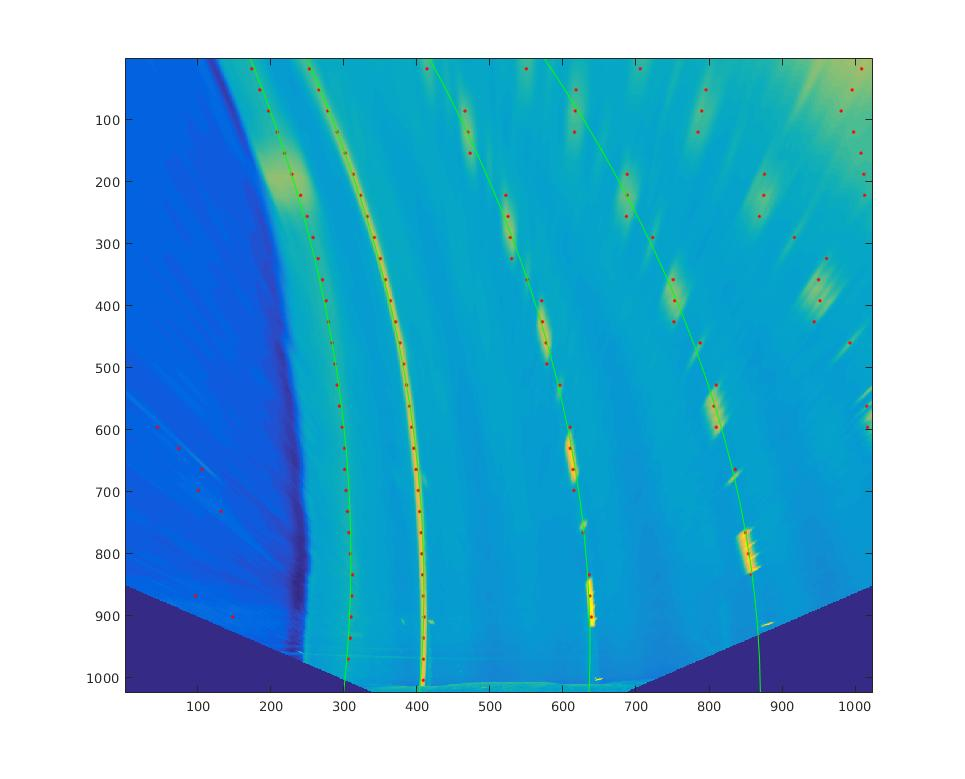
\includegraphics[width=1.0\linewidth]{img/road}
    \caption{IPM output along with lane markers and fitted polynomials}
    \label{fig_ipm}
\end{figure}


\section{Traffic Sign Detection}

To find traffic signs I use two simple RGB color normalization formulas, for blue and red. In addition I use the saturation value from the HSV color space. That turns out to be a pretty good predictor for signs since they tend to have very bright, saturated colors. This classifier reliably finds most signs, but unfortunately it also picks up a lot of noise. To reduce some of the false positives I set some restrictions on the size and aspect ratio of objects.

To classify traffic signs I use an SVM model trained with HOG features for each sign. The features I use are obtained by first resizing sign image to $60 \times 60$ pixels, which is then split into 9 $20 \times 20$ sub-images. For each sub-image I generate 3 histograms for hue, saturation and gradient direction, each with 10 bins. This produces 270 dimensional feature vector. This model got about 85\% accuracy on the test set, decent but not amazing.

 My traffic sign detector produces a lot of false positives and I had hoped that the classifier could be the last step in filtering them out, unfortunately the scores returned by my classifier give no indication whether the object is noise or a real sign.

\end{document}